\section{簡介}
多語言句法剖析希望借助多種語言的句法訓練資料互相增進彼此語言的分析正確率。
前人文獻指出對齊不同語言的詞表示有助於語言間的\zeroshot\cite{cao2020multilingual}。
本研究則提出使用\XNorm,透過在批次內進行\XNorm的方式拉近不同語言詞表示之平均與標準差,
以達到類似對齊不同語言的效果。
曹氏(Steven Cao)提出的對齊法\cite{cao2020multilingual}使用需要平行語料,
屬於較為細緻的對齊法,
但現存的依存句法剖析樹庫缺少大量語言的平行語料,
唯一的平行句法樹庫PUD(Parallel Universal Dependencies)被UD句法樹庫置於測試集中,
且多為常見語言,對資料不足語言的幫助有限,
因此\XNorm只在批次層級試圖匹配不同語言的統計性質,嘗試在沒有平行語料的幫助下達到類似對齊的效果,
以增進未見過的語言的分析正確率。

\section{使用\XNorm在依存句法剖析}
\subsection{批次\XNorm(Batch Normalization)}
批次\XNorm為瑟氏(Sergey Ioffe)在2015年提出\cite{pmlr-v37-ioffe15},
其認為其中一個深層類神經網路難以訓練的原因為每層輸入的分佈由於前層參數的調整一直在變動,
這使得深層類神經網路的訓練需要較小的學習率,也因此使訓練時間變長,
瑟氏稱此現象為內部共變量偏移(internal covariate shift);
因此他提出\XNorm每層的輸入,使輸入的分佈變動幅度變小,學習率得以提高,模型表現對初始參數也較不敏感,
大幅減少訓練時間(所需時間僅使用批次\XNorm之前的十四分之一),
並在發表時刷新了ImageNet圖像辨識\cite{Deng2009ImageNetAL}的辨識率記錄。

給定輸入 $x$ ,輸出 $y$ ,批次\XNorm層運作如下:
\begin{equation}
    y = \frac{x - \mathbb{E}[x]}{\sqrt{\textrm{Var}[x] + \epsilon}}
\end{equation}
其中 $\epsilon$ 是防止分母為0所加上的微小數值。
如此一來,輸出 $y$ 的平均變爲0,方差變為1,順利解決了內部共變量偏移的問題;
但單單對輸入做\XNorm會改變該層可以代表的函數集合,
%舉例來說,若對S函數的輸入做\XNorm,\XNorm後的數值將全部落在S函數的線性區間中。
為了確保加了批次\XNorm後的網路的表現力與加入前相同,
瑟氏提出的批次\XNorm還加入了額外的縮放參數 $\gamma$ 與偏差參數 $\beta$ :
\begin{equation}
    y = \frac{x - \mathbb{E}[x]}{\sqrt{\textrm{Var}[x] + \epsilon}} \times \gamma + \beta
\end{equation}
當$\gamma = \textrm{Var}[x]$,$\beta = \mathbb{E}[x]$時,該層網路即回復到與未加批次\XNorm前的網路有相同的行為。
\subsection{語言\XNorm(Language Normalization)}
在多語言的場景下,本節欲探討對齊不同語言分佈的方法會為模型在訓練語言與未見過的語言帶來什麼樣的改變。

令$\mathcal{L}_{train}$ 為所有訓練語言的集合,語言\XNorm的運作如下:
\begin{equation}
    y = \frac{x - \mathbb{E}[x]}{\sqrt{\textrm{Var}[x] + \epsilon}}
    \times \gamma_{\ell} + \beta_{\ell},\ \forall \ell \in \mathcal{L}
\end{equation}
其中 $\ell \in \mathcal{L}_{train}$ 為欲進行\XNorm運算的語言, $\gamma_{\ell}$ 與 $\beta_{\ell}$ 分別為該語言的縮放與偏差參數。


\vspace{12pt}
\noindent\textbf{加入語言\XNorm的多語言適應器$\mathrm{mBERT}$}
\vspace{4pt}

\section{使用領域對抗式訓練在依存句法剖析}
\begin{figure}[h]
    \centering
    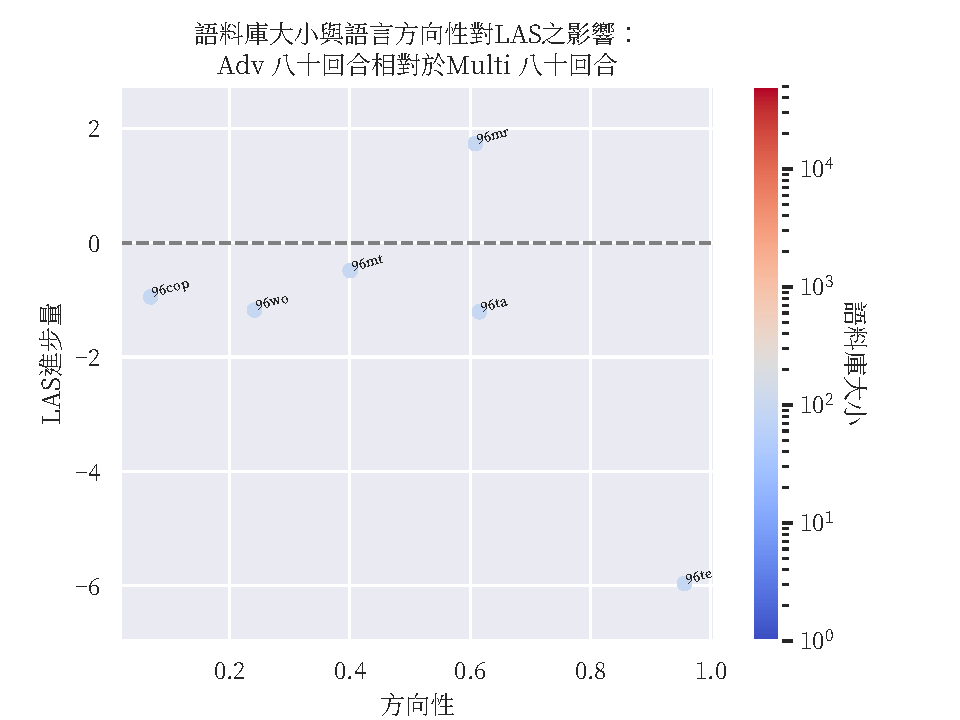
\includegraphics{figs/chapter4/adv_to_multi.pdf}
    \caption{方向性與句法樹庫大小對領域對抗式訓練模型相對於基準模型各自進行單語言\finetune後LAS之進步量的影響}
    \label{fig:dir-size-las-ft-fomaml-to-multi}
\end{figure}
\section{相關研究}
%\section{使用在依存句法剖析}
\section{實驗設置}
%\subsection{\zeroshot(Zero-shot Transfer)}
%\subsection{精細校正(Fine-tuning)}
%\section{實驗結果}
%\subsection{\zeroshot(Zero-shot Transfer)}
%\subsection{精細校正(Fine-tuning)}
